\chapter{Introduction}
\section{Main Idea}

\section{Objectives and Scope of Thesis}

\section{Review of Existing Solutions}

Two similar solutions exist in Poland. Both of them are represented in Figure 1. One was explicitly created for the University of Warsaw. We draw inspiration from it to include some functionalities like news feed and mailbox in our project. Unlike the first app, the second one can show data for more than one university. Users have to choose what university they attend, and then they can see their calendar, grades, and some other data from the chosen university system. This is what we wanted to achieve while designing our application. Most of our attention went to creating a simple and extensible API. The program represented in the document was designed to provide better user experience than the second solution described here, and it is supposed to be easily expendable by YAML files and also new widgets and views.

% TODO - ask if I can use these graphics and how to link them
% TODO - zeobić doagram przepływów i opisac kazdy wireframe i jak kiedzy nimy przechodzic
\begin{figure}[htb]
    \centering
    \begin{tabular}{@{}ll@{}}
        a) & b) \\
        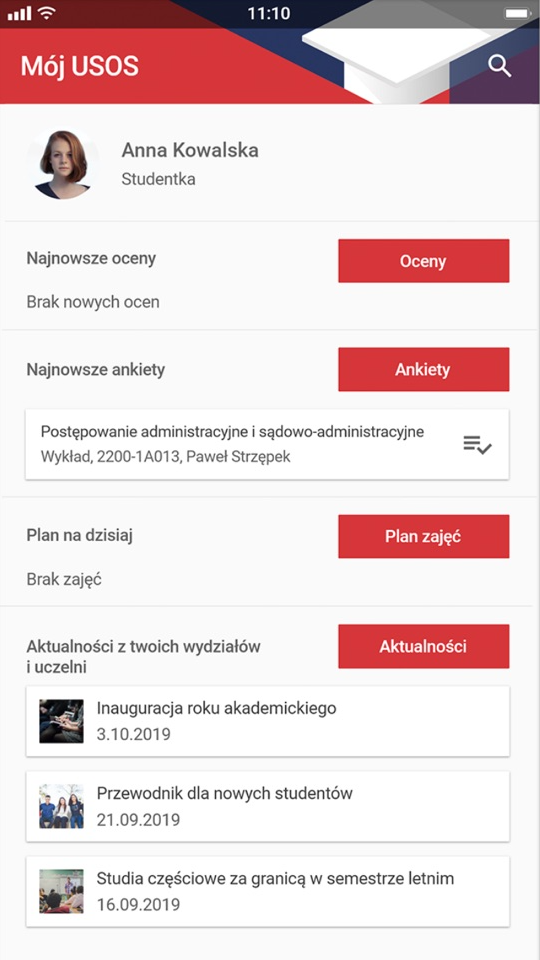
\includegraphics[width=0.425\textwidth]{fig01/mobilny-usos.png} &
        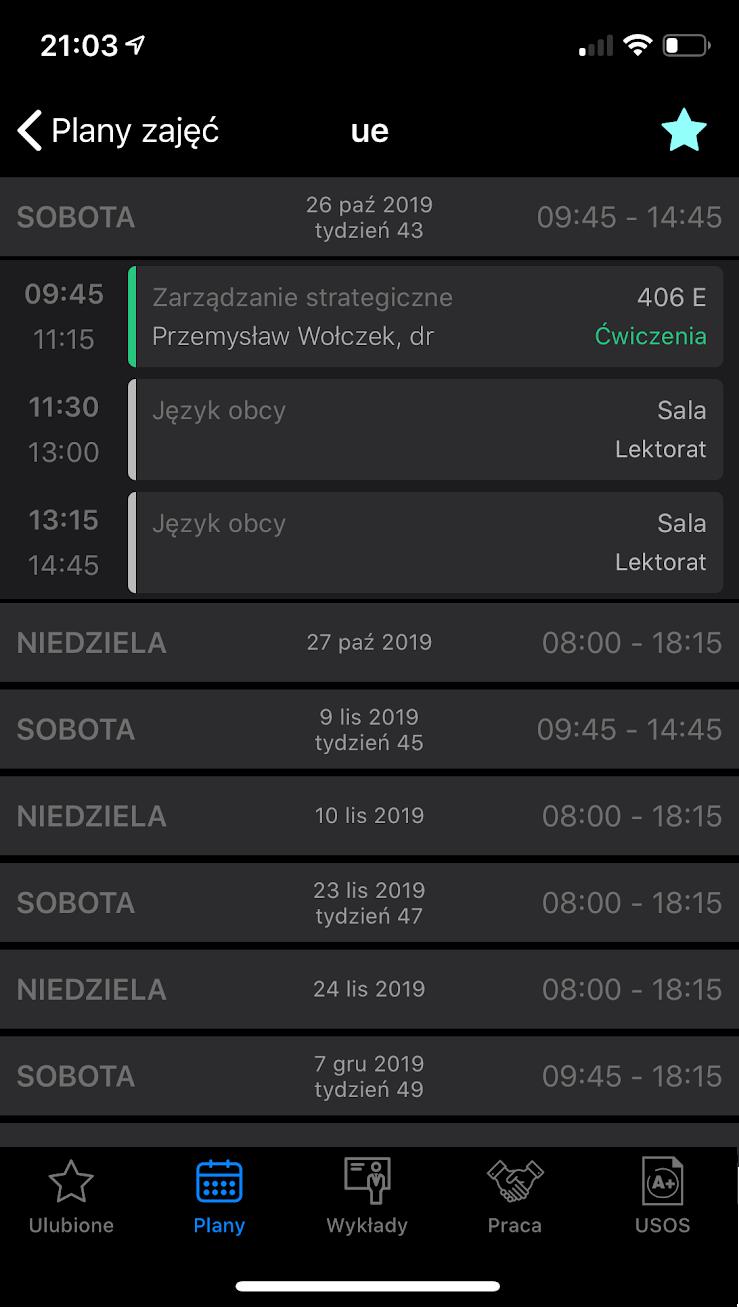
\includegraphics[width=0.425\textwidth]{fig01/kiedy-wyklad.png} \\
    \end{tabular}
    \caption{Similar solutions existing in Poland: a) Mobilny USOS UW, b) Kiedy wykład} \label{fig:similiar-solutions}
\end{figure}

\section{Thesis Structure}
